\chapter{Using color separation as a stellar characterization tool}\label{chap:color_as_tool}
% TEXT ==========================================

\section{Color probability density functions}

\section{Applicability to modern surveys}
Therefore J is just damn special, and it would be a subject of future work as to why J band spectral features are gravity sensitive for GKM dwarfs (J-K for M dwarfs) and J-W1/2 for GK dwarfs.

We also note the importance the J-band is in differentiating between dwarfs from giants given its previously proved sensitivity for differentiating M dwarfs from GK dwarfs for J-K (REF). The combination of this study with J-W1/2 in being sensitive for GK dwarfs, and J-K being sensitive for GKM stars suggests the presence of surface gravity sensitive lines in the J-band. Thus, there we suggest it is viable to search for gravity sensitive lines along these the J-band wavelength range.

% FIGURES ==========================================

\begin{figure}
    \centering
    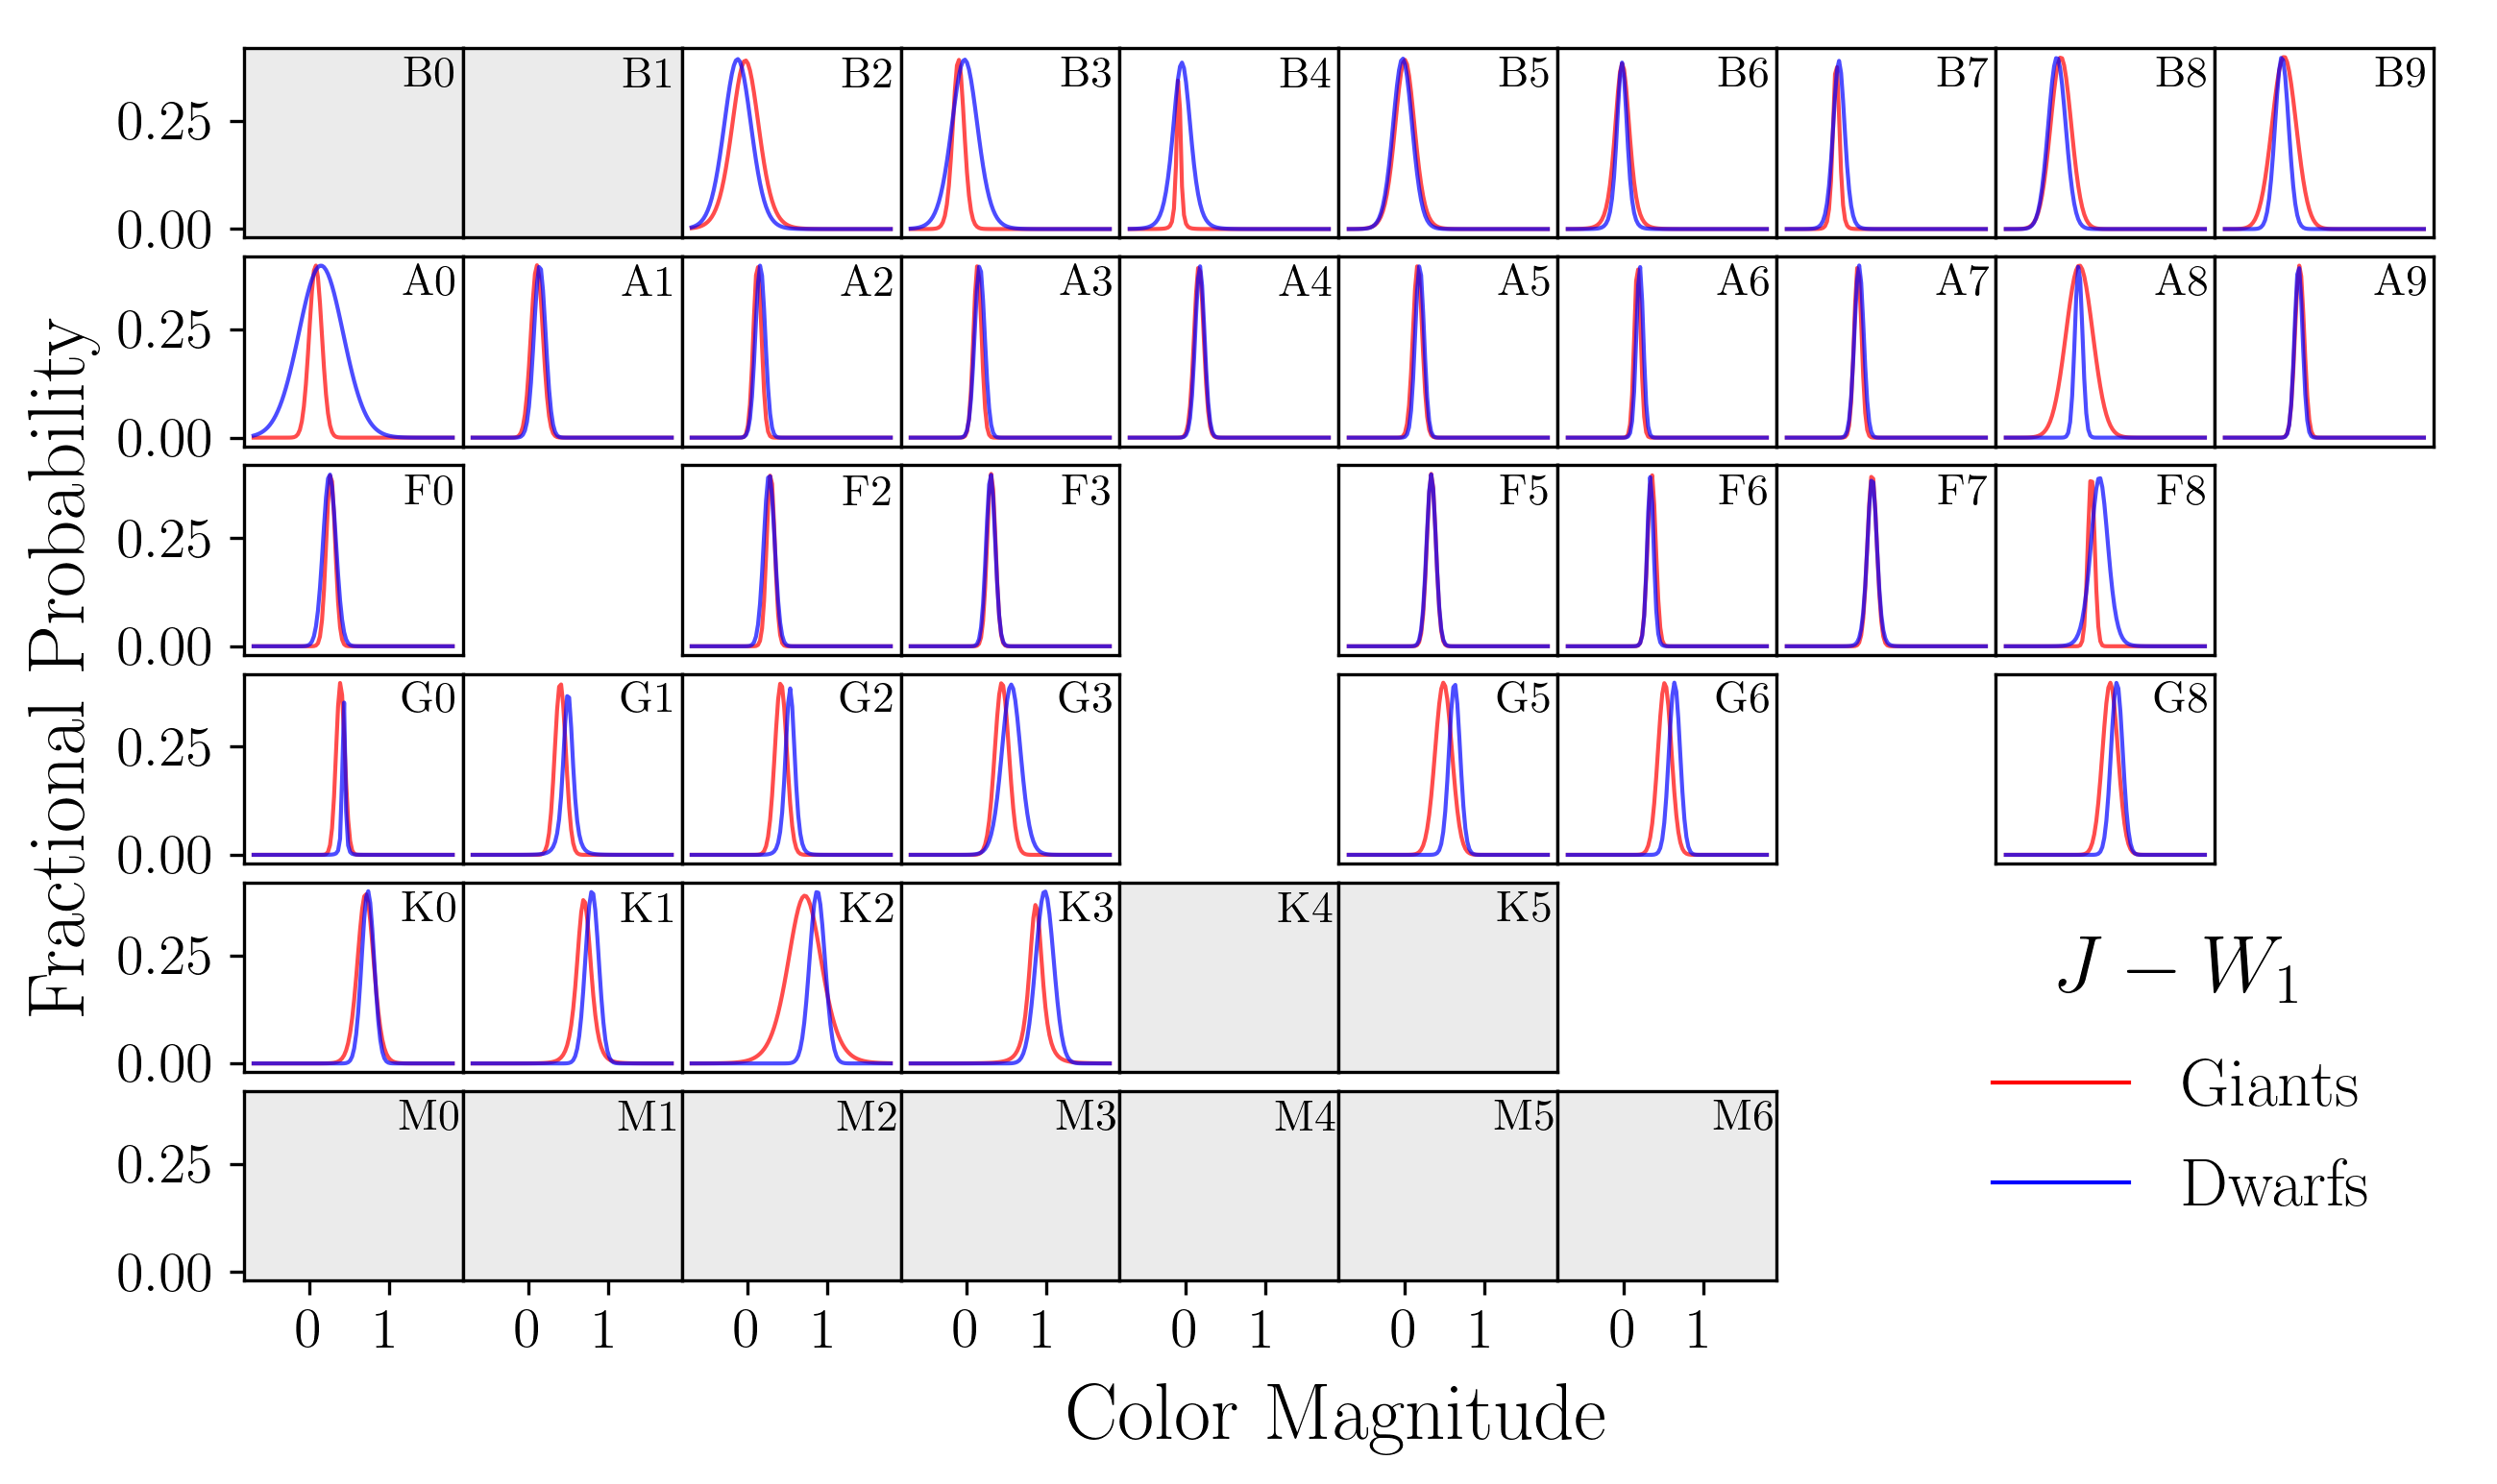
\includegraphics[width=1.0\textwidth,clip=true]{Figures/periodic/periodic-t-pdf_J_W1.png}
    \caption{Caption}
    \label{fig:periodic-pdf-jw1}
\end{figure}

\begin{figure}
    \centering
    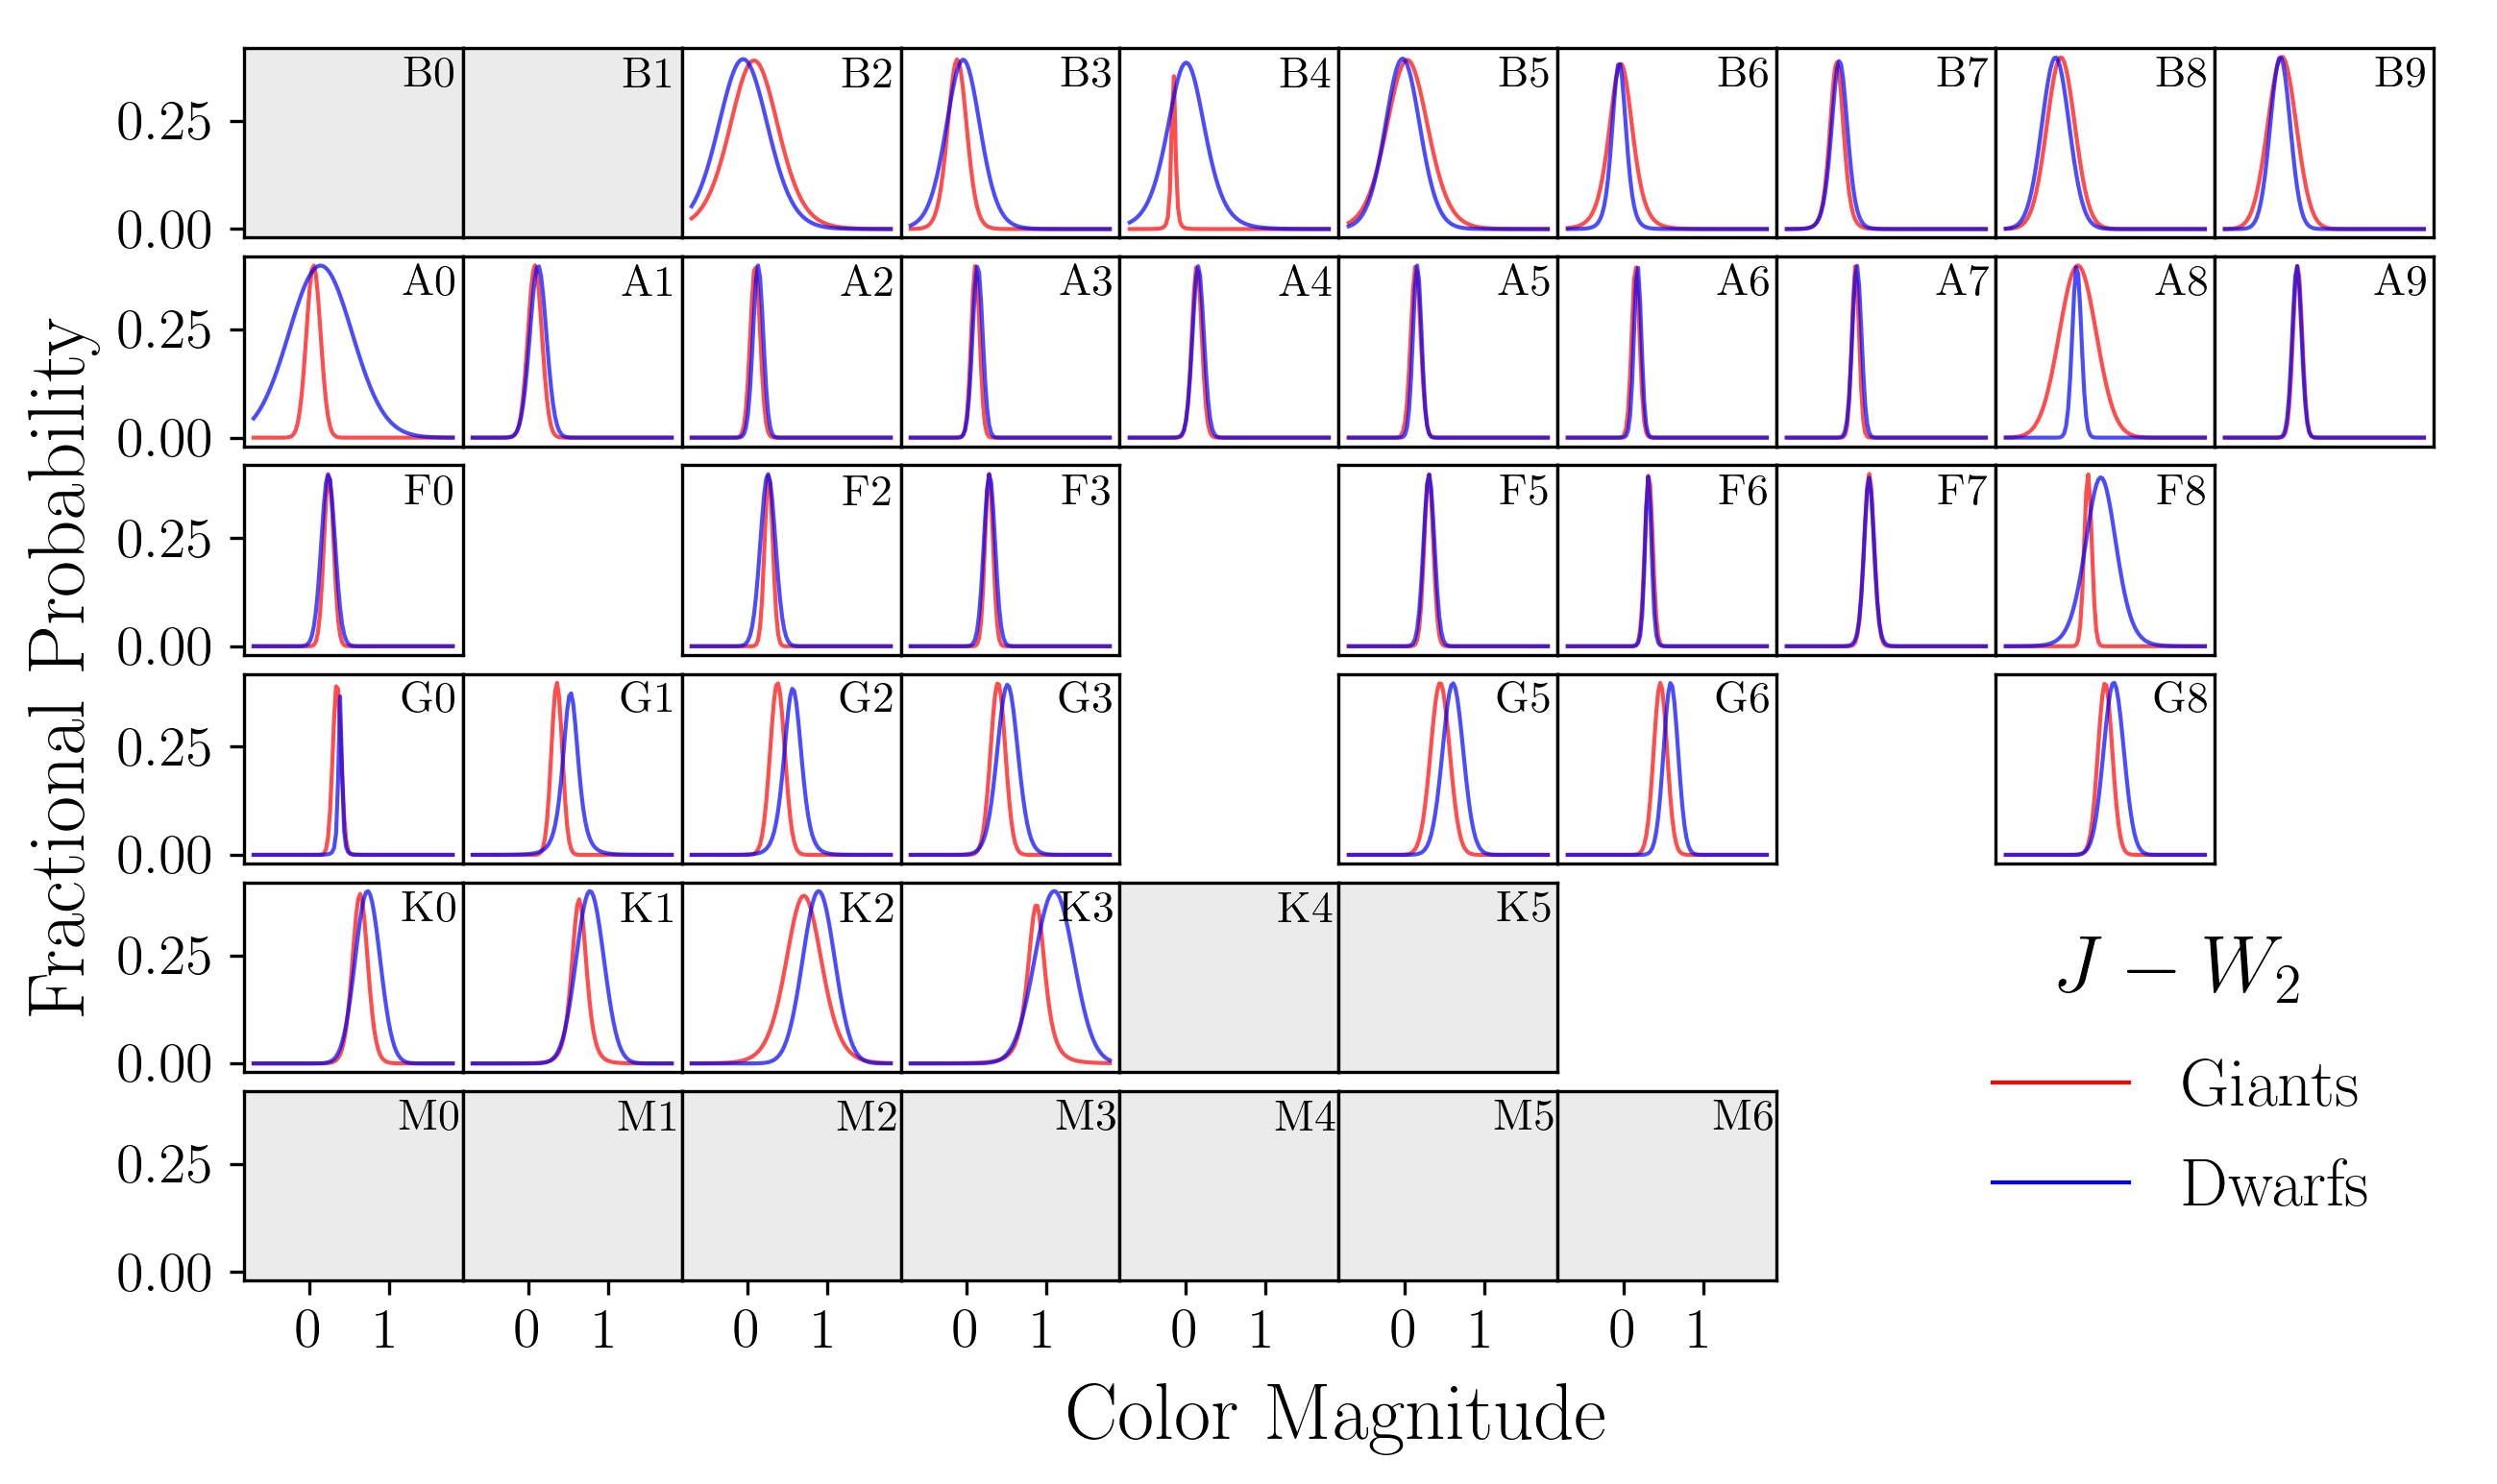
\includegraphics[width=1.0\textwidth,clip=true]{Figures/periodic/periodic-t-pdf_J_W2.png}
    \caption{Same as Figure \ref{fig:periodic-pdf-jw1}, but for \jwtwo.}
    \label{fig:periodic-pdf-jw2}
\end{figure}

\begin{figure}
    \centering
    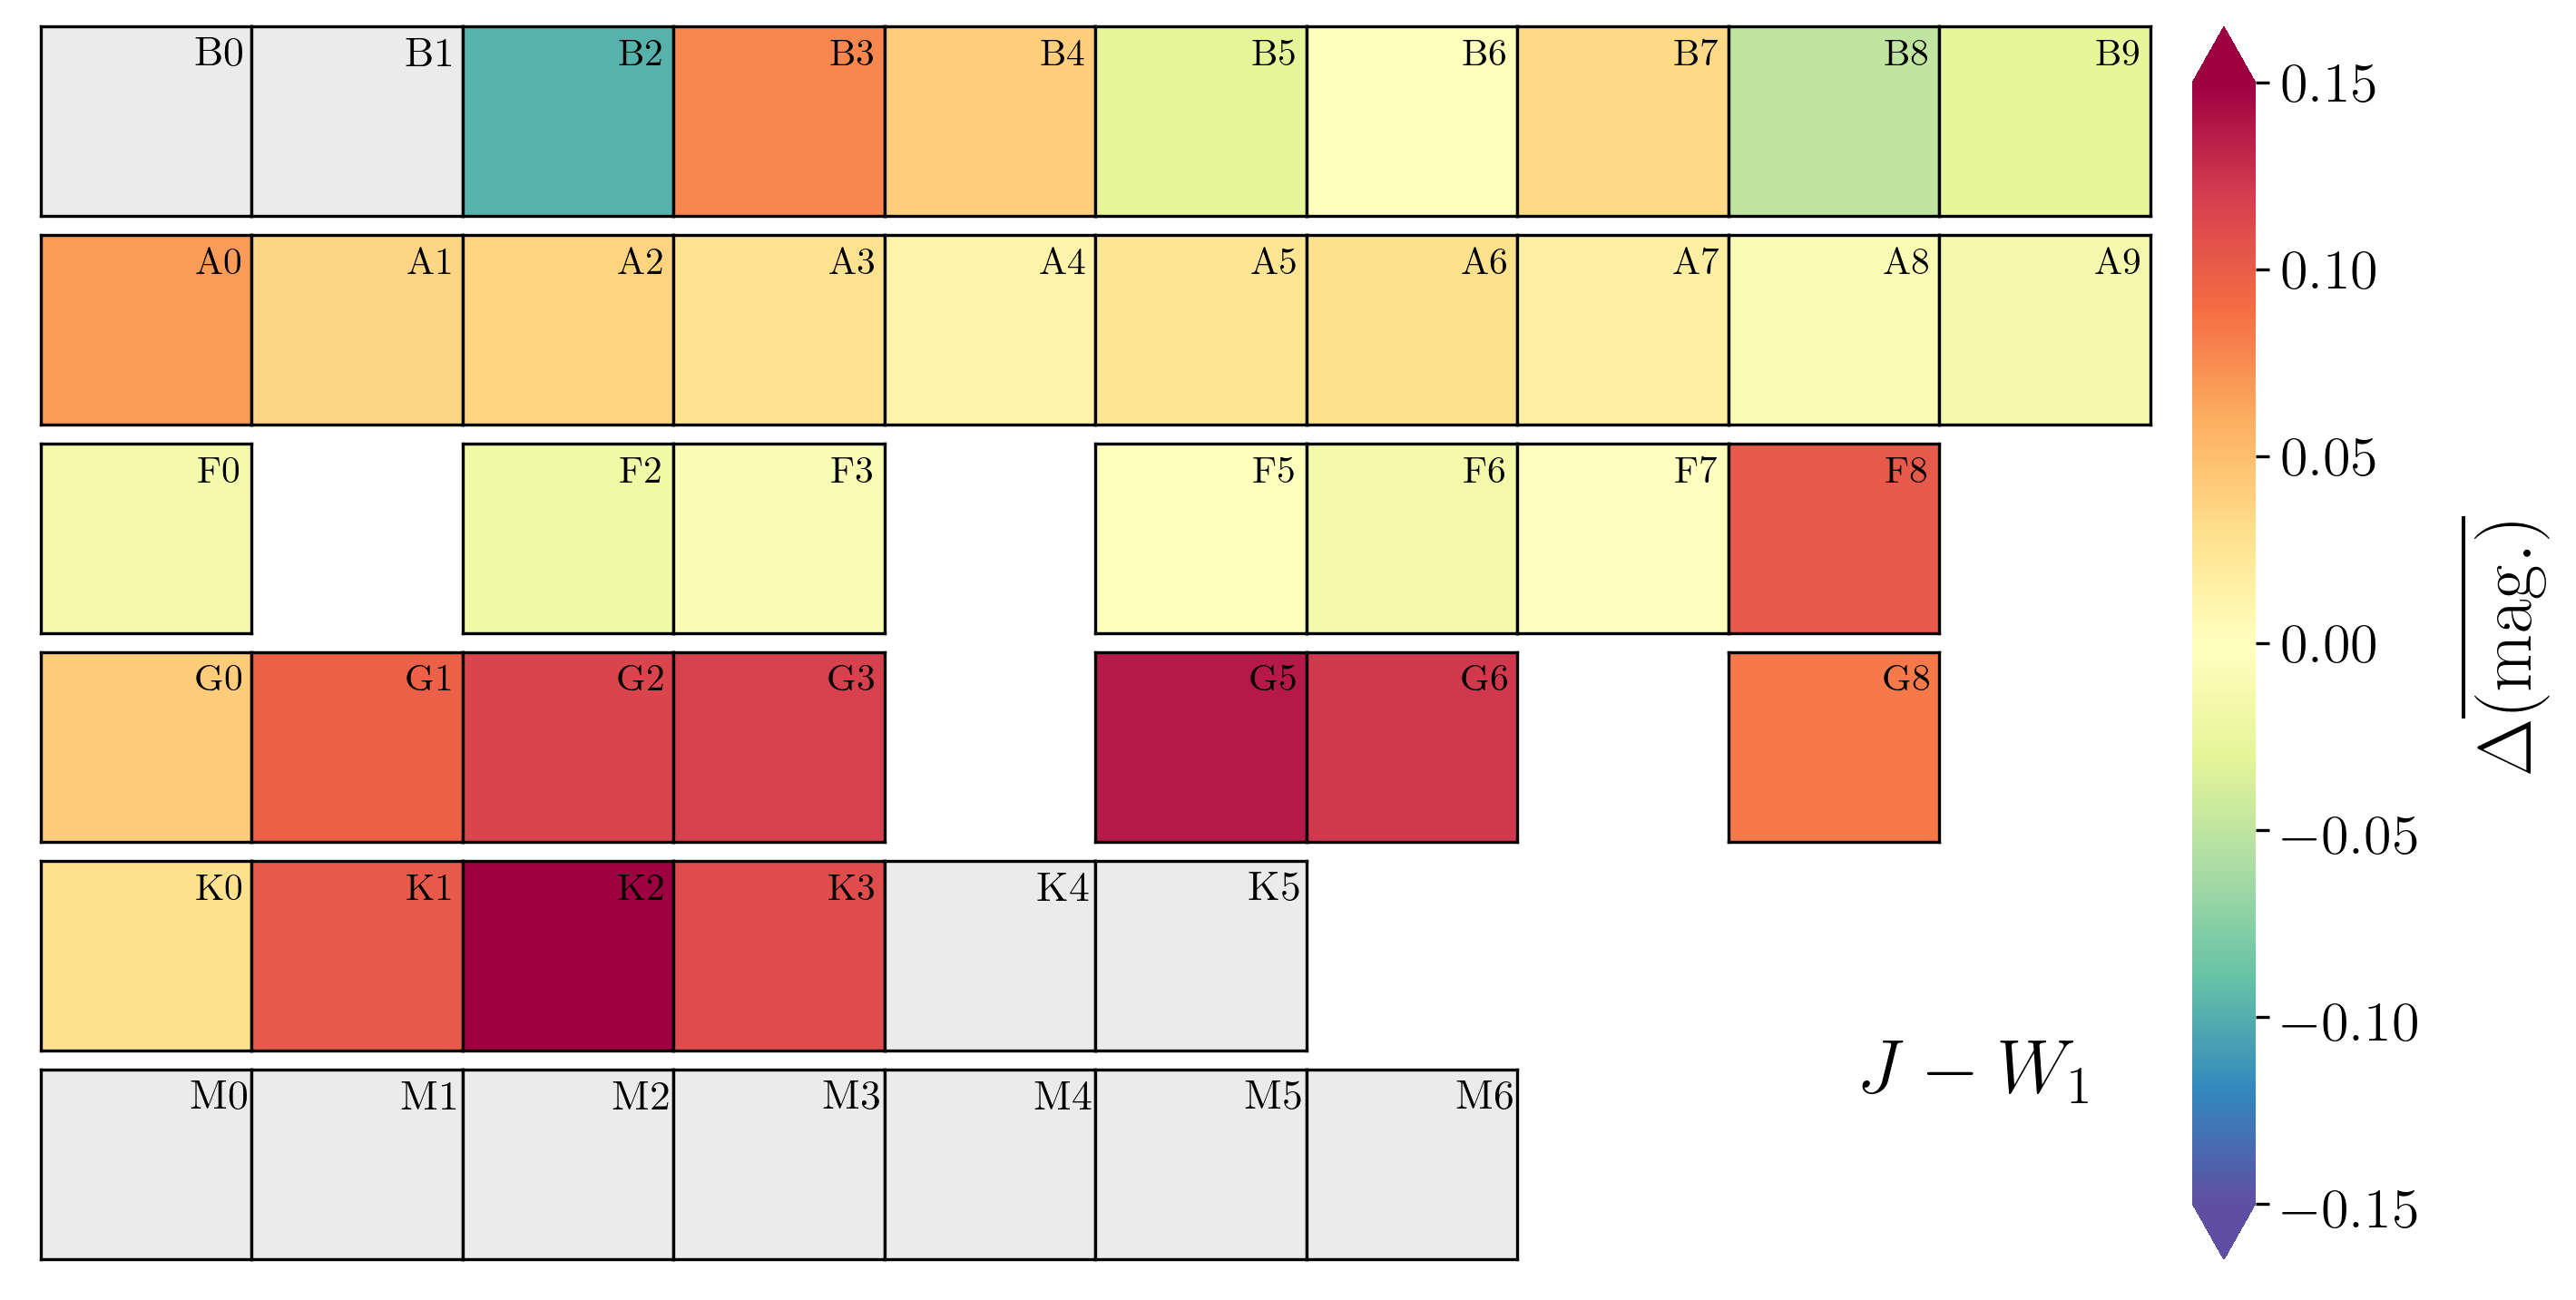
\includegraphics[width=1.0\textwidth,clip=true]{Figures/periodic/periodic-delta_J_W1.png}
    \caption{Caption}
    \label{fig:periodic-delta-jw1}
\end{figure}

\begin{figure}
    \centering
    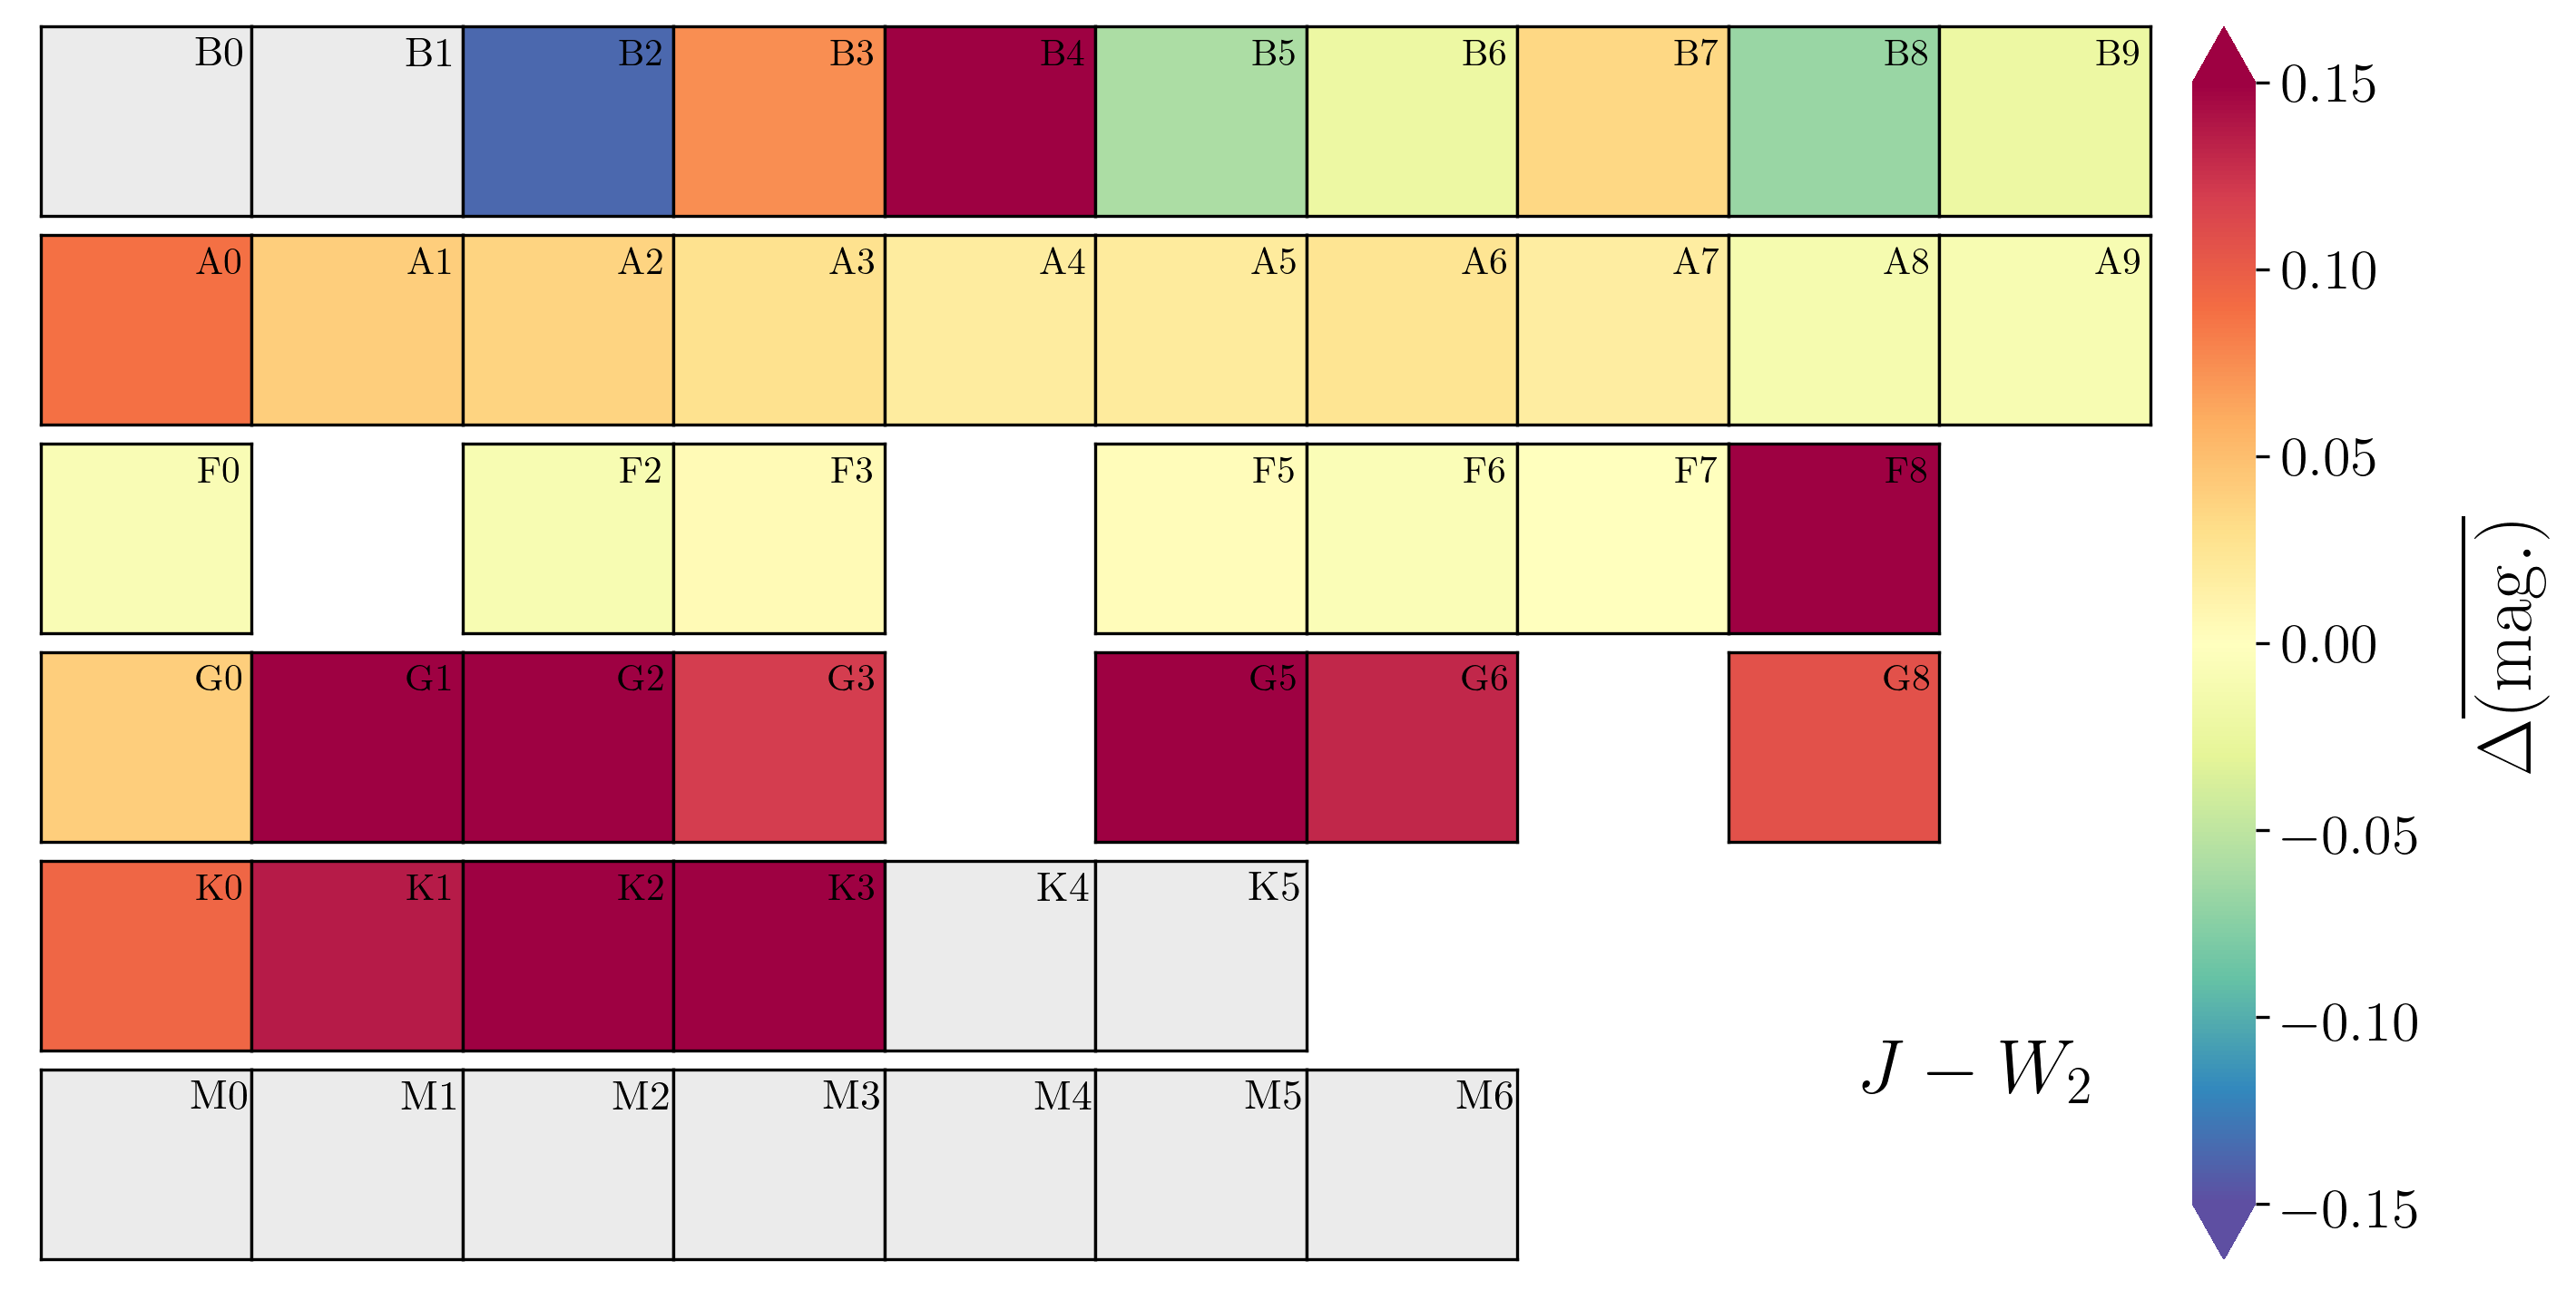
\includegraphics[width=1.0\textwidth,clip=true]{Figures/periodic/periodic-delta_J_W2.png}
    \caption{Same as Figure \ref{fig:periodic-delta-jw1}, but for \jwtwo.}
    \label{fig:periodic-delta-jw2}
\end{figure}
